\documentclass{article}
\usepackage[utf8]{inputenc}
\usepackage{hyperref}
\usepackage{csquotes}
\usepackage{graphicx}

\graphicspath{ {res/} }
\hypersetup{
    colorlinks=true,
    linkcolor=none,
    urlcolor=magenta,
}

\renewcommand{\familydefault}{\sfdefault}
\newcommand{\chikalegal}{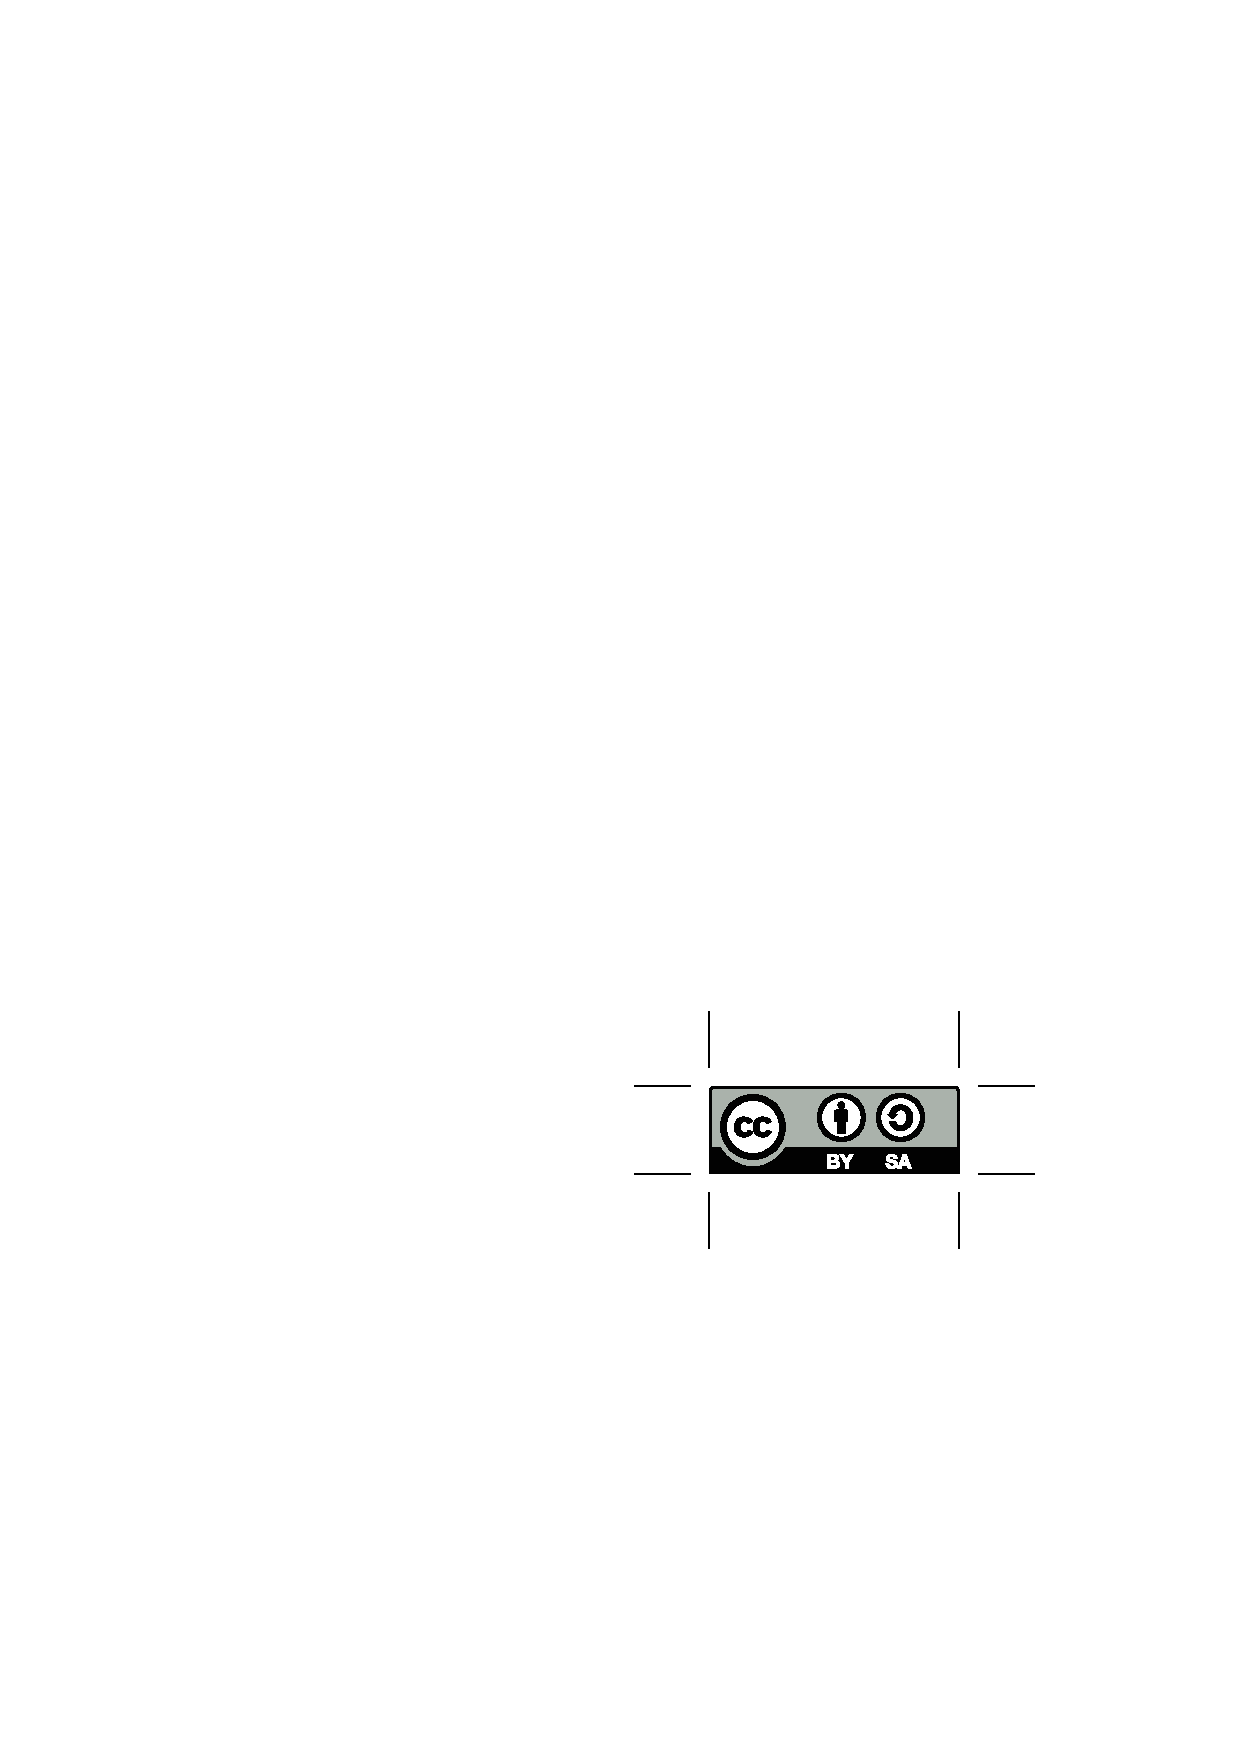
\includegraphics[scale=0.75]{by-sa}

This work is licensed under the Creative Commons Attribution-ShareAlike 4.0 International License. To view a copy of this license, visit \url{http://creativecommons.org/licenses/by-sa/4.0/} or send a letter to Creative Commons, PO Box 1866, Mountain View, CA 94042, USA. Copyright \copyright~2019-\the\year~Chika Games.

The RPG Maker trademark and copyright are property of Enterbrain, Inc. and Kadokawa Corporation. All rights belong to their respective owners.}
\newcommand{\specpreamble}{\maketitle
\tableofcontents
\newpage
\chikalegal
\newpage}


\title{LCF Map Tree Specification (LMT)}
\author{Chika Games}

\begin{document}
\specpreamble

\section{Introduction}
LCF Map Tree files are used to store map properties, game start information, and map orderings for RPG Maker 2000/2003 games.

This specification is part of a larger collection that can be found at the following URL: \url{https://github.com/chika-games/RPG-Maker-Specifications}.

\section{Data Types}
\subsection{Basic Data Types}
\subsubsection{Encoded Integers}
\subsection{Compound Data Types}
\subsubsection{STRING Type}

\section{LMT File Structure}
\subsection{Example Map Hierarchy}
\section{Map Info Structure}
\section{Map Start Structure}

\section{Tags}
\subsection{Map Info Tags}
\subsection{Map Start Tags}
\subsection{Music Tags}
\subsection{Encounter Tags}

\end{document}
